% $Header$

\documentclass[aspectratio=1610]{beamer}

\mode<presentation>
{%
  \usetheme{Boadilla}
}


\usepackage[english]{babel}
\usepackage[utf8]{inputenc}
\usepackage[T1]{fontenc}

\usepackage{%
    animate,
    graphicx,
    varwidth,
    tcolorbox,
    clrscode3e,
    tikz,
    mathtools,
    forest,
}
\usetikzlibrary{shapes.multipart, trees, overlay-beamer-styles, positioning, calc}

\tikzset{%
    block/.style={%
        font=\sffamily,
        draw=black,
        thin,
        fill=pink!50,
        rectangle split,
        rectangle split horizontal,
        rectangle split parts=#1,
        outer sep=0pt
    },
    gblock/.style={%
        block,
        rectangle split parts=#1,
        fill=green!30
    },
    invisible/.style={opacity=0},
    visible on/.style={alt={#1{}{invisible}}},
    alt/.code args={<#1>#2#3}{%
      \alt<#1>{\pgfkeysalso{#2}}{\pgfkeysalso{#3}} % \pgfkeysalso doesn't change the path
    },
    every node/.style={draw, circle, minimum size=.5cm, scale=0.5},
    edge from parent/.style={draw},
    level distance=1cm,
    level 1/.style={sibling distance=5em},
    level 2/.style={sibling distance=2.5em},
    % level 3/.style={sibling distance=1em}
    bchild/.style={draw,thick}, % bold child
    %
    % red-black trees
    every br node/.style={%
        shape=circle, text width=width("00"), align=center, text=white,
        font=\bfseries\large, minimum size=1cm, scale=1
    },
    bnode/.style={every br node, fill=black},
    rnode/.style={every br node, fill=red},
}

\forestset{%
  on slide/.style args={<#1>#2}{/tikz/alt=<#1>{#2}{}},
  declare boolean={bnode}{true},
  rnode/.style={not bnode},
  br tree/.style={%
    delay={%
      where content={}{%
        every br node, fill=none,
        edge+={draw=none},
      }{%
        if bnode={/tikz/bnode}{/tikz/rnode},
        alias/.option=content,
      },
    },
    % for tree={%
    %   calign=fixed edge angles,
    % },
  },
}

\graphicspath{{../../imgs/rbt/}}

% alert a whole line (especially for algorithms)
\newcommand{\alertline}{%
 \usebeamercolor[fg]{normal text}%
 \only{\usebeamercolor[fg]{alerted text}}}

% floor command
\newcommand{\floor}[1]{\left\lfloor #1 \right\rfloor}

\title[ALG25 - Lecture 6]
{Red-Black Trees}

\subtitle
{Algorithms and Datastructures, F25, Lecture 6}

\author[Andreas H. Høeg-Petersen]
{Andreas Holck Høeg-Petersen}

\institute[AAU]{%
  Department of Computer Science\\
  Aalborg University
}

\date {\today}

\pgfdeclareimage[height=0.5cm]{university-logo}{../../imgs/aau-logo}
\logo{%
    \begin{tikzpicture}[overlay,remember picture]
        \node[left=0.2cm] at (current page.30){\pgfuseimage{university-logo}};
    \end{tikzpicture}
}

\AtBeginSection[]
{%
  \begin{frame}<beamer>{Outline}
    \tableofcontents[currentsection,currentsubsection]
  \end{frame}
}


\begin{document}

\begin{frame}
  \titlepage
\end{frame}

\begin{frame}{Opdateringer}{}
    \begin{itemize}[<+->]
        \small
        \item Næste programmeringsopgave er ude --- har I alle set den?
            \begin{itemize}
                \item Der vil være lidt ekstra tid til exercises i dag, og det
                    er blandt andet, så I eventuelt kan arbejde lidt med opgaven
            \end{itemize}
    \end{itemize}
\end{frame}


\begin{frame}{Outline}
  \tableofcontents
\end{frame}


\section{Introduktion til Red-Black Trees}

\begin{frame}{Recap}{Udfordringer ved BST'er}
    Vi så til sidste forelæsning på binære søgetræer

    \begin{itemize}[<+(1)->]
        \item De var super seje
        \item De understøttede alle vores elskede operationer ---
            $\proc{Insert}$, $\proc{Delete}$, $\proc{Search}$,
            $\proc{Maximum}$/$\proc{Minimum}$ og lignende --- og kunne gøre det
            i $\log n$ tid
        \item Eller det vil sige\ldots
            \begin{itemize}
                \item Alle procedurerne kørte i tid proportionelt med træets
                    højde $h$
                \item For et \alert{balanceret} træ med $n$ knuder har vi at $h
                    = \Theta(\log n)$
                \item Men i worst case er $h = n$
            \end{itemize}
        \item Kan vi gøre noget ved det?
    \end{itemize}
\end{frame}


\begin{frame}{Bedre tider}{See what I did there??}
    \begin{figure}[h]
        \centering
        \includegraphics[width=0.8\textwidth]{../yes-we-can}
    \end{figure}
\end{frame}



\begin{frame}{Red-Black Trees}{Egenskaber}
    Vi introducerer nu en ny datastruktur, som er en lettere modificeret udgave
    BST'er. \pause

    \begin{itemize}[<+(1)->]
        \item Alle knuder indeholder nu også en attribut $\id{color} \in \{
            \const{RED}, \const{BLACK} \}$
        \item Vi repræsenter nu blade som $\const{NIL}$-pointers (så alle knuder
            med nøgler er `interne knuder')
        \item Et red-black tree er et BST, som overholder følgende
            \alert{red-black egenskaber}:
            \begin{enumerate}
                \item Alle knuder er enten røde eller sorte
                \item Roden er sort
                \item Alle blade er er sorte
                \item Hvis en knude er rød, så er begge dens børn sorte
                \item Alle simple stier fra en knude til et blad i et af dets
                    subtræer indeholder den samme mængde sorte knuder
            \end{enumerate}
        \item Vi kalder antallet af sorte knuder på en simpel sti fra en knude
            $x$ (eksklusiv $x$ selv) til et blad for knudes `sorte højde',
            $\id{bh}(x)$
    \end{itemize}
\end{frame}

\begin{frame}{Red-Black Trees}{Illustrationer}
    \begin{figure}[h]
        \centering
        \includegraphics<1>[width=0.8\textwidth]{rbt-a}
        \includegraphics<2>[width=0.8\textwidth]{rbt-b}
        \includegraphics<3>[width=0.8\textwidth]{rbt-c}
    \end{figure}

    \only<1>{Et RBT hvor alle blade er sorte $\const{NIL}$-knuder}
    \only<2>{Vi bruger en \alert{sentinel} $\const{NIL}$-knude til at
    repræsentere alle blade (og forældren til roden)}
    \only<3>{Men vi gider ikke tegne det hver gang, så man skal bare huske, at
    der egentlig altid er pointers til disse sorte $\const{NIL}$-knuder}
\end{frame}


\begin{frame}{Red-Black Trees}{Garanti for højden}
    Med disse egenskaber på plads kan vi garantere, at højden for et RBT med $n$
    interne knuder højst er $2 \log(n+1)$, hvilket er i $O(\log n)$. Hvorfor?

    \begin{proof}<2->[Lemma 13.1: Højden på et RBT er højst $2\log(n+1)$]
        \begin{itemize}[<+(1)->]
            \item Først, bemærk at et sub-træ med rod i en knude $x$ har mindst
                $2^{bh(x)}-1$ interne knuder
            \item Dernæst, det følger af den 4. egenskab (en rød knude skal have
                2 sorte børn), at mindst halvdelen af knuderne på enhver sti fra
                roden til et blad er sorte
            \item Det giver os
                \begin{align*}
                    n&\geq 2^{h/2} - 1 \\
                    n+1&\geq 2^{h/2} \\
                    \log(n+1)&\geq h/2
                \end{align*}
            \item Hvilket vi også kan skrive som $h \leq 2 \log(n+1)$
        \end{itemize}
    \end{proof}
\end{frame}


\begin{frame}{Rotationer}{Basal operation}
    Eftersom insertion og deletion laver ændringer i træet, skal vi bruge en
    basal operation kaldet $\proc{Left-Rotate}$\footnote{%
        Eller tilsvarende, $\proc{Right-Rotate}$.
    } til at rette op på de eventuelle brud med RBT-egenskaberne.
    \medskip

    \begin{columns}
        \column{.66\textwidth}
        \begin{columns}
            \column{.4\textwidth}<4->
            \centering
            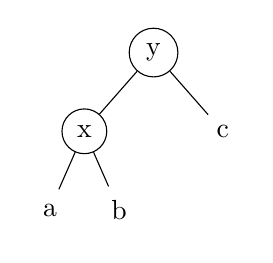
\begin{tikzpicture}[
                every node/.style={draw, circle, scale=1},
                ]
                
                \node {y}
                    child {node {x}
                        child {node[draw=none] {a}}
                        child {node[draw=none] {b}}
                    }
                    child {node[draw=none] {c}};
            \end{tikzpicture}

            \column{.2\textwidth}
            \footnotesize
            \centering

            \uncover<3->{%
                $\proc{Left-Rotate}(T,x)$\\
                $\longleftarrow$
            }

            \bigskip

            \uncover<6->{%
                $\proc{Right-Rotate}(T,y)$\\
                $\longrightarrow$ 
            }
        
            \column{.4\textwidth}<2->
            \centering
            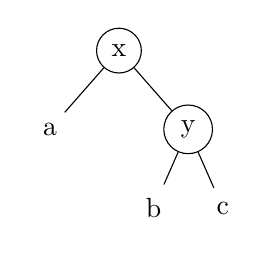
\begin{tikzpicture}[
                every node/.style={draw, circle, scale=1}
                ]
                \node {x}
                    child {node[draw=none] {a}}
                    child {node {y}
                        child {node[draw=none] {b}}
                        child {node[draw=none] {c}}
                    };
            \end{tikzpicture}
        \end{columns}

        \bigskip
        \uncover<5->{%
            $\proc{Left-Rotate}$ udnytter, at hvis $x$ er $y$s mor, så er alt i
            $y$s venstre sub-træ stadig større end $x$ og kan dermed gøres til
            $x$s højre barn, mens $x$ selv kan gøres til $y$s nye venstre barn.
        }
        
        \column{.33\textwidth}
        \begin{block}{$\proc{Left-Rotate}(T,x)$}
            \footnotesize
        
            \vspace{-\abovedisplayskip}
            \begin{codebox}
                \li $y \gets \attrib{x}{right}$ 
                \li $\attrib{x}{right} \gets \attrib{y}{left}$
                \li \If $\attrib{y}{left} \neq \attrib{T}{nil}$ \Then
                \li     $\attribb{y}{left}{p} \gets x$ 
                    \End
                \li $\attrib{y}{p} \gets \attrib{x}{p}$ 
                \li \If $\attrib{x}{p} \isequal \attrib{T}{nil}$ 
                    \Then
                \li     $\attrib{T}{root} \gets y$
                \li \ElseIf $x \isequal \attribb{x}{p}{left}$ 
                    \Then
                \li     $\attribb{x}{p}{left} \gets y$ 
                \li \Else $\attribb{x}{p}{right} \gets y$
                    \End
                \li $\attrib{y}{left} \gets x$ 
                \li $\attrib{x}{p} \gets y$ 
            \end{codebox}
        \end{block}
    \end{columns}
\end{frame}


\begin{frame}{Rotationer}{Left-Rotate}
    \begin{figure}[h]
        \centering
        \includegraphics[width=0.7\textwidth]{left-rotate}
    \end{figure}
\end{frame}


\section{Insertion i Red-Black trees}


\begin{frame}{Insertion}{}
    Med rotationer på plads er vi klar til at se på, hvordan insertion virker i
    et RBT.\ Vi starter med at sammenligne med insertion for almindelige BST'er:

    \begin{columns}[t]
        \scriptsize

        \column{.45\textwidth}
         \begin{block}{$\proc{Tree-Insert}(T,z)$}
        
            \vspace{-\abovedisplayskip}
            \begin{codebox}
                \li $x \gets \attrib{T}{root}$ 
                \li $y \gets \const{NIL}$ 
                \li \While $x \neq \const{NIL}$  
                    \Do
                \li     $y \gets x$ 
                \li     \If  $\attrib{z}{key} < \attrib{x}{key}$ 
                        \Then
                \li         $x \gets \attrib{x}{left}$
                \li     \Else $x \gets \attrib{x}{right}$
                        \End
                    \End

                \li $\attrib{z}{p} \gets y$ 

                \li \If $y \isequal \const{NIL}$ 
                    \Then
                \li     $\attrib{T}{root} \gets z$ 
                \li \ElseIf $\attrib{z}{key} < \attrib{y}{key}$ 
                    \Then
                \li     $\attrib{y}{left} \gets z$
                \li \Else $\attrib{y}{right} \gets z$
                    \End
                \li
                \li
                \li
                \li
            \end{codebox}
        \end{block}       
    
        \column{.45\textwidth}
        \begin{block}{$\proc{RB-Insert}(T,z)$}
        
            \vspace{-\abovedisplayskip}
            \begin{codebox}
                \li $x \gets \attrib{T}{root}$ 
                \li $y \gets \attrib{T}{nil}$ 
                \li \While $x \neq \attrib{T}{nil}$ 
                    \Do
                \li     $y \gets x$ 
                \li     \If $\attrib{z}{key} < \attrib{x}{key}$ 
                        \Then
                \li         $x \gets \attrib{x}{left}$
                \li     \Else $x \gets \attrib{x}{right}$ 
                        \End
                    \End
                \li $\attrib{z}{p} \gets y$ 
                \li \If $y \isequal \attrib{T}{nil}$
                    \Then
                \li     $\attrib{T}{nil} \gets z$ 
                \li \ElseIf $\attrib{z}{key} < \attrib{y}{key}$ 
                    \Then
                \li     $\attrib{y}{left} \gets z$
                \li \Else $\attrib{y}{right} \gets z$
                    \End
                \li $\attrib{z}{left}\gets \attrib{T}{nil}$
                \li $\attrib{z}{right} \gets \attrib{T}{nil}$ 
                \li $\attrib{z}{color} \gets \const{RED}$
                \li $\proc{RB-Insert-Fixup}(T,z)$
            \end{codebox}
        \end{block}
    \end{columns}
\end{frame}

\begin{frame}{Insertion}{Violations}
    Nu er spørgsmålet, hvilke af RBT-egenskaberne kan ødelægges ved insertion?

    \begin{columns}[t]

        \column{.55\textwidth}
        \begin{enumerate}[<+(1)->]
            \item Alle knuder er enten røde eller sorte
                \begin{itemize}
                    \footnotesize
                    \item \alert{Nej} - alle knuder er fortsat røde eller sorte
                \end{itemize}
            \item Roden er sort
                \begin{itemize}
                    \footnotesize
                    \item \alert{Ja} - hvis træet er tomt, så bliver den nye,
                        røde knude roden
                \end{itemize}
            \item Alle blade er er sorte
                \begin{itemize}
                    \footnotesize
                    \item \alert{Nej} - den nye knude har $\attrib{T}{nil}$
                        (sort) som blade/børn
                \end{itemize}
            \item Hvis en knude er rød, så er begge dens børn sorte
                \begin{itemize}
                    \footnotesize
                    \item \alert{Ja} - hvis den nye knudes mor er rød
                \end{itemize}
            \item Alle simple stier fra en knude til et blad i et af dets
                subtræer indeholder den samme mængde sorte knuder
                \begin{itemize}
                    \footnotesize
                    \item \alert{Nej} - den nye knude er rød og bidrager dermed
                        ikke til den sorte højde
                \end{itemize}
        \end{enumerate}

        \column{.35\textwidth}
        \scriptsize
        \begin{block}{$\proc{RB-Insert}(T,z)$}
        
            \vspace{-\abovedisplayskip}
            \begin{codebox}
                \li $x \gets \attrib{T}{root}$ 
                \li $y \gets \attrib{T}{nil}$ 
                \li \While $x \neq \attrib{T}{nil}$ 
                    \Do
                \li     $y \gets x$ 
                \li     \If $\attrib{z}{key} < \attrib{x}{key}$ 
                        \Then
                \li         $x \gets \attrib{x}{left}$
                \li     \Else $x \gets \attrib{x}{right}$ 
                        \End
                    \End
                \li $\attrib{z}{p} \gets y$ 
                \li \If $y \isequal \attrib{T}{nil}$
                    \Then
                \li     $\attrib{T}{nil} \gets z$ 
                \li \ElseIf $\attrib{z}{key} < \attrib{y}{key}$ 
                    \Then
                \li     $\attrib{y}{left} \gets z$
                \li \Else $\attrib{y}{right} \gets z$
                    \End
                \li $\attrib{z}{left}\gets \attrib{T}{nil}$
                \li $\attrib{z}{right} \gets \attrib{T}{nil}$ 
                \li $\attrib{z}{color} \gets \const{RED}$
                \li $\proc{RB-Insert-Fixup}(T,z)$
            \end{codebox}
        \end{block}
    \end{columns}
\end{frame}


\begin{frame}{Fiks insertions}{$\proc{RB-Insert-Fixup}$}
    Vi ser nu på $\proc{RB-Insert-Fixup}$ proceduren, der genopretter
    RBT-egenskaberne efter insertion:

    \begin{columns}
        \column{.5\textwidth}
        \begin{block}{$\proc{RB-Insert-Fixup}(T,z)$}
            \footnotesize
        
            \vspace{-2\abovedisplayskip}
            \begin{codebox}
                \li \While $\attribb{z}{p}{color} \isequal \const{RED}$
                    \Do
                \li     \If $\attrib{z}{p} \isequal
                            \attrib{\attribb{z}{p}{p}}{left}$
                        \Then
                \li         $y \gets
                                \attrib{\attribb{z}{p}{p}}{right}$ 
                \li         \If $\attrib{y}{color} \isequal \const{RED}$ 
                            \Then
                \li             $\attribb{z}{p}{color} \gets \const{BLACK}$ 
                \li             $\attrib{y}{color} \gets \const{BLACK}$ 
                \li             $\attrib{\attribb{z}{p}{p}}{color} \gets \const{RED}$ 
                \li             $z \gets \attribb{z}{p}{p}$
                \li         \Else
                \li             \If $z \isequal
                                    \attribb{z}{p}{right}$ 
                                \Then
                \li                 $z \gets \attrib{z}{p}$
                \li                 $\proc{Left-Rotate}(T,z)$
                                \End
                \li             $\attribb{z}{p}{color} \gets
                                    \const{BLACK}$ 
                \li             $\attrib{\attribb{z}{p}{p}}{color}
                                    \gets \const{RED}$
                \li             $\proc{Right-Rotate}(T,
                                    \attribb{z}{p}{p})$
                            \End

                \li     \Else same, but swap `left' and `right'
                        \End
                    \End
                \li $\attribb{T}{root}{color} \gets \const{BLACK}$ 

            \end{codebox}
        \end{block}
    
        \column{.5\textwidth}
        \only<1-5>{%
            \begin{itemize}[<+->]
                \item $z$ er rød, så vi går kun ind i while-løkken, hvis dens
                    mor også er rød
                \item Vi tjekker, om $z$'s mor er et venstre barn
                \item Hvis $z$'s moster ($y$) er rød, så skal både den og $z$'s
                    mor farves sorte, mens bedstefar gøres rød --- og vi fortsætter
                    nu fra bedstefar
                \item Hvis moster ikke var rød, og $z$ er et højre barn, så skal vi
                    lave en $\proc{Left-Rotate}$
                \item Var $z$ venstre barn laver vi en $\proc{Right-Rotate}$
            \end{itemize}
        }
        
        \only<6->{%
        \begin{center}
            \begin{forest}
            br tree,
            [11,
            on slide= <12->{rnode},
            on slide=<13->{rnode, before typesetting nodes = {%
                replace by=7,
                prepend=8,
              },
            },
              [7,
              on slide=<7-10>{rnode},
              on slide=<-9>{before typesetting nodes = {%
                    replace by=!1,
                    delay n=2{%
                      prepend=5,
                    },
                  },
                },
              on slide=<13->{before typesetting nodes = {%
                  replace by=2,
                  delay ={append=11,prepend=2},
                },
              },
                [2,rnode
                  [1
                    [,draw=none]
                    [,draw=none]
                  ]
                  [5,
                  on slide= <6>{rnode},
                  on slide=<-9>{before typesetting nodes={%
                        delay = {replace by=7}, 
                      },
                    },
                    [4,rnode]
                    [,draw=none]
                  ]
                ]
                [8, on slide= <6>{rnode}
                    [,draw=none]
                    [,draw=none]
                ]
              ]
              [14, bnode
                [,draw=none]
                [15, rnode]
              ]
            ]
            %
            \node<6>  [draw=none,anchor=east] at (4.west)  {\Large $z$};
            \node<-7> [draw=none,anchor=west] at (8.east)  {\Large $y$};
            \node<7-8>[draw=none,anchor=east] at (7.west)  {\Large $z$};
            \node<8-> [draw=none,anchor=west] at (14.east) {\Large $y$};
            \node<9-> [draw=none,anchor=east] at (2.west)  {\Large $z$};
            \end{forest}
        \end{center}
        }
    \end{columns}
\end{frame}


\section{Exercises}

\begin{frame}{Exercises}{Super fedt! <3}

    På Moodle! Go! Fungerer det fint?

    \begin{figure}[h]
        \centering
        \includegraphics[width=0.8\textwidth]{../exercises}
    \end{figure}
    
\end{frame}


\section{Deletion i RBT}

\begin{frame}{Deletion i RBT}{Mere komplekst}
    Vi vender nu blikket mod det at skulle slette et element $z$ fra et RBT.

    \begin{itemize}[<+(1)->]
        \item Ligesom for binære søgetræer er det en noget mere kompliceret
            procedure
        \item Der er modificeret udgave af $\proc{Transplant}$-proceduren ---
            kaldet $\proc{RB-Transplant}$ --- som ligesom for BST'er erstatter
            en knude $u$ med en anden knude $v$
        \item Til at genoprette RBT-egenskaberne efter deletion findes der en
            procedure $\proc{RB-Delete-Fixup}$
            \begin{itemize}
                \item Den kommer vi ikke til at gå ind i
            \end{itemize}
    \end{itemize}
\end{frame}


\begin{frame}{Deletion}{}

    \begin{columns}[t]
        \column{.45\textwidth}
        \only<2>{%
            \begin{block}{$\proc{Tree-Delete}(T,z)$}
                \scriptsize

                \vspace{-1.5\abovedisplayskip}
                \begin{codebox}
                    \li
                    \li
                    \li \If $\attrib{z}{left} \isequal \const{NIL}$ 
                    \Then
                    \li
                    \li     $\proc{Transplant}(T,z,\attrib{z}{right})$
                    \li \ElseIf $\attrib{z}{right} \isequal \const{NIL}$ 
                    \Then
                    \li
                    \li     $\proc{Transplant}(T,z,\attrib{z}{left})$
                    \li \Else 
                    $y \gets \proc{Tree-Minimum}(\attrib{z}{right})$ 
                    \li
                    \li
                    \li     \If $y \neq \attrib{z}{right}$
                    \Then
                    \li         $\proc{Transplant}(T,y,\attrib{y}{right})$
                    \li         $\attrib{y}{right} \gets \attrib{z}{right}$ 
                    \li         $\attribb{y}{right}{p} \gets y$ 
                    \li
                    \End
                    \li     $\proc{Transplant}(T,z,y)$
                    \li     $\attrib{y}{left} \gets \attrib{z}{left}$
                    \li     $\attribb{y}{left}{p} \gets y$ 
                    \End
                    \li
                    \li
                    \li

                \end{codebox}
            \end{block}
        }
        \only<3->{%
            \begin{itemize}[<+(3)->]
                \footnotesize
                \item Som i $\proc{Tree-Delete}$ vil vi slette knude $z$
                \item Linie 1-8 tjekker om $z$ kun har 1 barn, og erstatter så
                    bare $z$ med det barn
                \item Hvis vi rammer linie 9, så har $z$ to børn, og vi finder
                    dets successor $y$
                \item I linie 12-15 tjekker vi, om $y$ er længere nede i træet
                    --- i så fald erstatter vi $y$ med dets højre barn, og lader
                    det derefter pege på $z$'s højre barn
                \item Herefter kan vi erstatte $z$ og $y$ med hinanden og give
                    $z$'s venstre barn til $y$ (som ikke havde et venstre barn,
                    da det er $z$'s successor i højre sub-træ)\footnote{%
                        \scriptsize
                        Bemærk at linie 16 er mærkelig, men er nødvendig for
                        $\proc{RB-Delete-Fixup}$ senere
                    }
                \item Til sidst tjekker vi, om farven på den knude, vi har
                    pillet ved (enten $z$ eller dens successor $y$) oprindeligt
                    var sort --- for så skal vi reparere træet!
            \end{itemize}
        }

        \column{.45\textwidth}
        \begin{block}{$\proc{RB-Delete}(T,z)$}
            \scriptsize
        
            \vspace{-1.5\abovedisplayskip}
            \begin{codebox}
                \li $y \gets z$ 
                \li $\id{yOrgColor} \gets \attrib{y}{color}$ 
                \li \If $\attrib{z}{left} \isequal \attrib{T}{nil}$
                    \Then
                \li     $z \gets \attrib{z}{right}$
                \li     $\proc{RB-Transplant}(T,z,\attrib{z}{right})$
                \li \ElseIf $\attrib{z}{right} \isequal \attrib{T}{nil}$
                    \Then
                \li     $x \gets \attrib{z}{left}$
                \li     $\proc{RB-Transplant}(T,z,\attrib{z}{left})$
                \li \Else
                        $y \gets \proc{Tree-Minimum}(\attrib{z}{right})$ 
                \li     $\id{yOrgColor} \gets \attrib{y}{color}$ 
                \li     $x \gets \attrib{y}{right}$
                \li     \If $y \neq \attrib{z}{right}$ 
                        \Then
                \li         $\proc{RB-Transplant}(T,y,\attrib{y}{right})$
                \li         $\attrib{y}{right} \gets \attrib{z}{right}$
                \li         $\attribb{y}{right}{p} \gets y$ 
                \li     \Else $\attrib{x}{p} \gets y$
                        \End
                \li     $\proc{RB-Transplant}(T,z,y)$
                \li     $\attrib{y}{left} \gets \attrib{z}{left}$
                \li     $\attribb{y}{left}{p} \gets y$
                \li     $\attrib{y}{color} \gets \attrib{z}{color}$
                    \End
                \li \If $\id{yOrgColor} \isequal \const{BLACK}$ 
                    \Then
                \li     $\proc{RB-Delete-Fixup}(T,x)$
                    \End
            \end{codebox}
        \end{block}
    \end{columns}
    
\end{frame}


\begin{frame}{Deletion}{Violations}
    Hvad kan gå galt?

    \begin{columns}
        \column{.5\textwidth}
        \begin{enumerate}[<+(1)->]
            \item Alle knuder er enten røde eller sorte
                \begin{itemize}
                    \footnotesize
                    \item \alert{Nej} - alle knuder er fortsat røde eller sorte
                \end{itemize}
            \item Roden er sort
                \begin{itemize}
                    \footnotesize
                    \item \alert{Ja} - hvis $z$ var roden og et rødt barn bliver
                        ny rod
                \end{itemize}
            \item Alle blade er er sorte
                \begin{itemize}
                    \footnotesize
                    \item \alert{Nej} - ingen blade skifter farve
                \end{itemize}
            \item Hvis en knude er rød, så er begge dens børn sorte
                \begin{itemize}
                    \footnotesize
                    \item \alert{Ja} - hvis $y$, da den blev flyttet, blev
                        erstattet af en rød knude
                \end{itemize}
            \item Alle simple stier fra en knude til et blad i et af dets
                subtræer indeholder den samme mængde sorte knuder
                \begin{itemize}
                    \footnotesize
                    \item \alert{Ja} - vi har fjernet en sort knude
                \end{itemize}
        \end{enumerate}

        \column{.4\textwidth}
        \begin{figure}[h]
            \centering
            \includegraphics<12>[width=0.8\textwidth]{delete-fixup}
        \end{figure}
    \end{columns}
\end{frame}


\begin{frame}{Reparere træet}{RB-Delete-Fixup}
    \begin{columns}
        \column{.45\textwidth}
        \begin{block}{$\proc{RB-Delete-Fixup}(T,x)$}
            \small
        
            \vspace{-\abovedisplayskip}
            \begin{codebox}
                \li \While $x \neq \attrib{T}{root}$ and $\attrib{x}{color}
                        \isequal \const{BLACK}$ 
                    \Do
                \li     \If $x \isequal \attribb{x}{p}{left}$ 
                        \Then
                \li         $w \gets \attribb{x}{p}{right}$
                \zi     \ldots
                \li     \Else \Comment Når $x \isequal \attribb{x}{p}{right}$ 
                \li         $w \gets \attribb{x}{p}{left}$ 
                \zi         \ldots
                        \End
                    \End
                \li $\attrib{x}{color} \gets \const{BLACK}$ 
            \end{codebox}
        \end{block}
    
        \column{.45\textwidth}
        \begin{itemize}[<+->]
            \item Proceduren tager træet $T$ og en knude $x$, som vi skal
                reparere fra
            \item Proceduren består af en while-løkke, som kører så længe, at
                $x$ ikke er roden og så længe, at $x$ er sort
            \item Koden består af 2 næsten identiske bidder, der kun adskiller
                sig ved, om $x$ er et venstre eller et højre barn
            \item $w$ angiver $x$'s søster
            \item Det hele slutter med, at vi farver $x$ sort
        \end{itemize}
    \end{columns}
\end{frame}


\begin{frame}{Reparere træet}{4 cases}
    Resten af koden håndterer 4 cases for, hvordan der kan være opstået
    problemer.

    \begin{figure}[h]
        \centering
        \includegraphics[width=0.45\textwidth]{delete-cases-12}
        \includegraphics[width=0.45\textwidth]{delete-cases-34}
    \end{figure}
\end{frame}


\begin{frame}{Reparere træet}{}
    \begin{center}
        Men fordi det \alert{næsten er fredag}, så gider vi ikke gå længere ind
        i det!
    \end{center}
\end{frame}


\begin{frame}{Tak for i dag!}{Flere exercises..}

    Den bedste måde ikke at snyde sig selv på er lave exercises!

    \begin{figure}[h]
        \centering
        \includegraphics[width=0.8\textwidth]{../exercises}
    \end{figure}
    
\end{frame}



\end{document}


